\documentclass[11pt]{article}
\usepackage{clrscode3e}
\usepackage{times}
\documentclass{article}
\usepackage{amssymb}
\usepackage{amsmath}
\usepackage{graphicx} % Required for inserting images
\usepackage[a4paper, total={7in, 10in}]{geometry}

\newcommand\cha{3}

\title{Capítulo \cha\   - Sutton}
\author{Paulo Henrique Albuquerque}
\date{2023-04-25}

\begin{document}

\maketitle

\textbf{Exercício \cha.1} 
\vspace{5mm}

\textbf{Solução.} 


\textbf{Exercício \cha.2} 
\vspace{5mm}

\textbf{Solução.} 

\textbf{Exercício \cha.3} 
\vspace{5mm}

\textbf{Solução.} 
\end{document}

\input{python}

\title
{
  Solving Gridworld with policy evaluation 

}

\begin{document}

\maketitle

\section{Introduction to the problem} 

We use the simple "GridWorld" problem as a model to test our policy evaluation algorithm.

The description of the problem is despicted bellow:

\begin{center}
\boxed{ 
  \begin{minipage}{\textwidth} \textbf{\textit{Problem Description.}} The left figure uses a rectangular grid to illustrate value functions for a simple finite {\color{blue}{MDP}}. 
The cells of the grid correspond to the states of the environment. 
At each cell, four actions are possible: {\color{blue} north, south, east,} and {\color{blue}west}, which deterministically cause the agent to move one cell in the respective direction on the grid. 
Actions that would take the agent off the grid leave its location unchanged, but also result in a reward of −1. Other actions result in a reward of 0, except those that move the agent out of the special states $A$ and $B$. From state $A$, all four actions yield a reward of +10 and take the agent to $A'$. 
From state $B$, all actions yield a reward of +5 and take the agent to $B'$ . Suppose the agent selects all four actions with equal probability in all states. 
The figure on the right shows the value function, $v_{\pi}$, for this policy, for the discounted reward case with {\color{red}$\gamma = 0.9$}. 
Notice the negative values near the lower edge; these are the result of the high probability of hitting the edge of the grid there under the random policy. 
State $A$ is the best state to be in under this policy, but its expected return is less than 10, its immediate reward, because from $A$ the agent is taken to $A'$ , from which it is likely to run into the edge of the grid. 
State $B$, on the other hand, is valued more than 5, its immediate reward, because from $B$ the agent is taken to $B'$ , which has a positive value. 
From $B'$ the expected penalty (negative reward) for possibly running into an edge is more than compensated for by the expected gain for possibly stumbling onto $A$ or $B$. 

\end{minipage} 
}
\end{center}

\begin{figure}[h]
  \begin{center}
    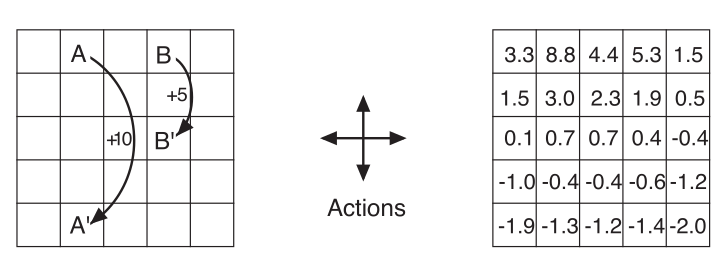
\includegraphics[width=0.6\textwidth]{../src/img/grid1.png}
  \end{center}
  \caption{States and value funcion for the gridworld}
  \label{fig:}
\end{figure}


Our objective is to get the same value function shown above using the policy evaluation algorithm.

\newpage

\section{The algorithm}

The policy evaluation algorithm in its simplest form is shown bellow:

\begin{codebox}
  \Procname{$\proc{Policy-Evaluation}(\pi)$}
  \li \Comment initialize a array $V[0 \twodots |S| - 1] \gets 0$ for all $s \in \mathcal{S}$ 
  \li \Repeat
  \li   $\Delta \gets 0$
  \li   \For each $s \in \mathcal{S}$   
  \li     \Do $\id{v} \gets V[s]$
  \li       $V[s] \gets \sum_{a}\pi(a|s)\sum_{s',r}p(s',r|s,a)[r+\gamma V[s']]$
  \li        $\Delta \gets \max{(\Delta,|\id{v}-V[s])}$
  \li     \End
  \li \Until $\Delta < \theta$ (a small positive number)
  \li \Return $V \approx v_{\pi}$
\end{codebox}

For deterministic policies, we can drop $\sum_{a} \pi(a|s)$ part on line 6 of \proc{Policy-Evaluation}.

In most cases, computing the $p(s',r|s,a)$ matrix is unfeasible (not in gridworld though). Instead, we "break" the process in two steps, and use the espected reward to simplify computations: 

\[v_{\pi}(s) = \sum_{a} \pi(a|s) \{r(s,a) + \gamma \sum_{s'} p(s'|s,a) v_{\pi}(s')}\]

In this form, we are left with a 2D matrix (to store $r(s,a)$ values) and a 3D matrix (to store $p(s',s,a)$ values), which simplifies the preprocessing drastically.

\subsection{Implementation}
We implemented the algorithm in Python. Check the code in https://github.com/paulohdosanjos/IC/sutton/cap4/gridworld.

\subsection{Results}
Running main.py, we get the following results:

\begin{figure}[h]
  \begin{center}
    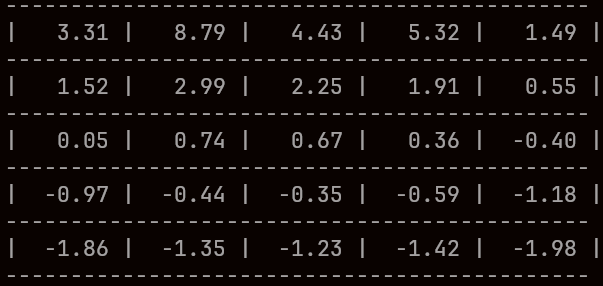
\includegraphics[width=0.6\textwidth]{../src/img/results.png}
  \end{center}
  \caption{Value function for the gridworld problem}
  \label{fig:}
\end{figure}


\end{document}
